\subsection{Result interpretation} \label{sec:analysisresults}
The data from the test covers three individual data types. 
Quantitative logging data, qualitative data consisting of observation notes and finally the interview notes.

\subsection{SOTA test interpretation}
The results obtained from the observation and interview concerning the SOTA controller will  not be subjected to grounded theory or any other interpretation, as the results were deemed of little relevance to any of the specified noteworthy subjects e.g. function delay, non responsiveness, activation difficulty, consecutive function difficulties and controller handling. The game play with the SOTA controllers was observed to not contain any cases of the observed notations or the questions as specified in the interview, and does therefore not include any of the difficulties as the constructed product contains.

\subsubsection{Observation notes}
As specified in the method chapter (\ref{sec:testcontent}), the observation notes are processed with the qualitative method of grounded theory which allows the data to be gathered into specified sets of data which can be subjected to form theories based upon the acquired material.



\subsection*{Open coding}
The observation notes consist of arrays of points for which the observations are noted in any random order as the observers wrote them down. 
Therefore, the first stage is to analyze the text and identify specific phenomena, and thereafter give each one a title for which the content will represent the phenomena. 
The method for which these are identified is with the use of researcher-denoted concepts. 
Since there exists no pre- established norms of how the content of the observation notes should be denoted, terms and instances which is deemed to emerge from the data is specified as headlines. 
This will make it possible to place each point into a specific constructed category. 
These categories will describe the underlying content.


The following categories are constructed to fit the observation notes.

\begin{itemize}
	\item Delay activating functions\newline
		Delay activating functions specifies the observation notes where the content has any relevance to any sort of delay 			which is observed, commented or experienced in game.
	\item Acceleration, Reverse/braking relevance\newline
		This headline covers all the observation notes that can be identified to contain data that emerge as difficulties 				with acceleration or reverse/braking during game play. 
	\item Change camera view relevance\newline
		The change camera view headline covers all the instances for which any notes have relevance to the camera view.
	\item Turning relevance\newline
		Turning relevance covers all of the notes that have any relevance to the turning mechanics. These comments can cover 			both game and controller mechanics.
	\item Subject comments \& actions\newline
		The subject comments and actions headline is for all comments that can be classified as test subject statements which 		are outspoken during gameplay. Additionally, test subject actions which are deemed noticeable and therefore commented 		are also placed here.
	\item Game \& in-game crashes\newline
		Covers the cases of in-game crashes and general game crashes that are specified as either controller malfunctioning 			or game difficulties that affect the test procedure.
	\item Frame rate relevance\newline
		Describes the observed incidents of reduced frame rate in game while playing.
\end{itemize}


\subsection*{Development of concepts}
The observation notes are thereafter identified and placed into the specific category that is deemed to be consistent and similar with the content. 
This method is utilized by color coding. (appendix: \ref{app:concept}))

\begin{figure}[!htbp]
\centering
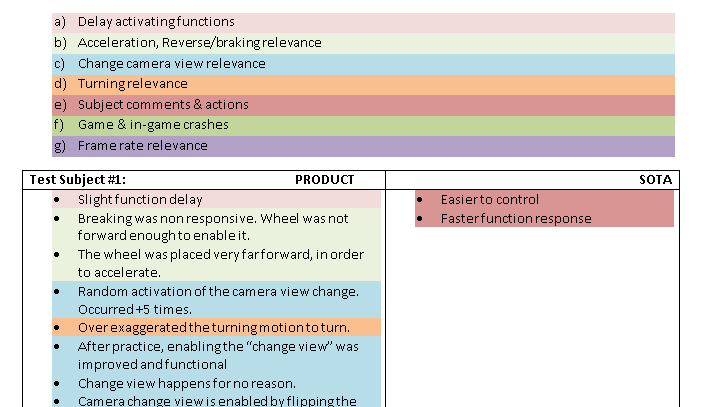
\includegraphics[scale=.5]{Eval1}
\caption{Color coding of the observation data} \label{fig:colorcoding}
\end{figure}

As seen on the figure (ref: Figure \ref{fig:colorcoding}), an example of the color coding of the notes is illustrated. 
By utilizing color coding, it is possible to ensure that each and every point of data is accounted for and placed into a specific category that fulfils the requirements for said category thus ensuring that the total amount of data is collected and placed accordingly.
\bigskip

The method for placing the content of the notes is by identifying the coding items that describes similar content to the categories that has been defined. 
Therefore it is possible to form groups of comments of similar content.
\bigskip

As an example of similar content (ref: figure \ref{fig:colorcoding}), the blue content being “change camera view relevance” under test subject \#1 is identified as similar content and therefore placed under that specific category.


\subsection*{Grouping concepts into categories}
 With the observation notes organized into relevant categories, it is now possible to identify broader groups of similar notes and identify those within each category that concludes upon the same data that might prove and explain relations and similarities.
 

The following subcategories cover the notes that have been identified within each category to describe or define similar indications of certain data elements which can be used to conclude upon the same subject.
\bigskip

For description of the categories and content, see appendix \ref{app:concept}.


\subsection*{Formation of a theory}
Now it is possible to formulate predictive interpretations of the specified data within each subcategory as defined and specified in the Grouping concepts into categories. 
Therefore the data is analyzed for what it indicates and what might be concluded by analyzing the explicit content of the connections or correlations of the content of each subcategory. If a specific title is not followed by subtitles, the content compliments only similar content.
\bigskip

\noindent\textbf{1. Delay activating functions}\newline
What can be interpreted from the responds is an indication of test subjects experiencing in-game delays of any sort. 
The delays can indicate to be one of two mentioned reasons:
\begin{itemize}
\item The delay from activating functions is caused by an actual delay from where any specific function is activated and a noticeable delay is occurring before any according respond is happening.
\item The other plausible cause is that the test subject accounts the actual movement of the controller as activation and does not take the time it takes for moving the controller to the “correct” location for activating the function into account. Thereby interpreting the movement, for which the controller is required to move in order to activate the function, as a function delay.
\end{itemize}
\bigskip

\noindent\textbf{2. Acceleration, Reverse/braking relevance}\newline


What can be interpreted and identified from the observations is that a problem concerning precision of placement of the controller is present, when the test subject is holding and controlling the product. 
A large amount of the test subjects was observed to have noticeable difficulties with the controls. 
What can be interpreted from the results is that the precision of the activation of controls must be more specified in terms of precision of the control placement in space, meaning that the functions has to be redefined so that the user is aware of exactly when and how to activate the desired functions.


The observation notes indicates that the movement of the controller which is necessary for any given function activation is too large/undefined causing unstable or irregular control of the specific functionalities.
\bigskip

\noindent \textbf{Game setting relevance}\newline
Not relevant to the product. Note describes issues with the game settings and not the product itself.
\bigskip

\noindent\textbf{3. Change camera view relevance}\newline
\bigskip

\noindent \textbf{Unintentional/accidental/unaccounted activation of the change camera setting}\newline


What can be interpreted from the notes is that a general inaccuracy of the change view function is apparent. 
Several notes indicate that the change view function is randomly occurring. 
This problem can be caused by one of several causes. 
Either the test subject is not handling the controller as it is supposed to, being the test subject moving the wheel too much left/right or up/down, accidentally activating the function. 
What is also apparent is the inaccurate method of activating the function, since the amount of notes indicates accidental activation.
\bigskip

\noindent \textbf{Active and intentional activation of the change camera setting}\newline


The notes indicates that the function for activating the change camera view is working as intended when correctly activated, but as previously discussed({\color{Red}3.1}) there are several issues with the specific function that causes difficulties.
\bigskip

\noindent \textbf{No activation of the change camera setting. Either optional or unsuccessful.}\newline

The following notes cannot be used to conclude upon anything. The notes specifies lap completions for which the change view was not enabled, and therefore represents test subject behavior and not product elements.

Additionally, the note that describes a test subject, trying to enable view where nothing occurred can indicate several plausible reasons, which cannot be concluded upon. 
Therefore the note will not be interpreted with plausible solutions.
\bigskip

\noindent\textbf{4. Turning relevance}\newline
\bigskip

\noindent \textbf{In-game steering difficulties: Overturning}\newline

The notes indicate that the test subjects find it hard to steer the product controller. 
What can be interpreted from the data is that the activation of turning which is utilized by keyboard presses causes difficulties.

The plausible reason is that the rotation of the wheel only activates a predefined amount of turning, as specified by the key press activation, where a wheel controller should perhaps be more likely to react accordingly to smaller gestures, resulting in small turns in game.
\bigskip

\noindent \textbf{Controller mechanics: Occasional unwilling turning} \newline

The notes indicate incidents where the subject experienced unwillingly turning right. 
Two plausible solutions could be causing the difficulties. 
The wheel controller utilizes BLOB’s to register the movement. 
The right BLOB on the product is blue. Coincidences of the webcam registering blue jeans or any other blue object which is larger than the desired blue object on the wheel, in the frame instead of the BLOB on the controller could result in accidental activation of turning right. 
Else, if the wheel was moved out of the frame of the webcam, another blue registered object might be subject to registration and cause the vehicle to turn in game.
\bigskip

\noindent\textbf{5. Subject comments \& actions}\newline
\bigskip

\noindent \textbf{Observed postures of the test subjects during gameplay.}\newline

The notes indicate that a large amount of the test subjects held the controller either very low or in straight arms close to the webcam.


A comment describes that the reason for holding controller very low, was tired arms. 
Another reason could be that the test subjects were unaware of the correct positioning of the wheel, since no detail of the correct placement is showed during the gameplay thus resulting in the subject holding the controller where he/she thinks that the controller should be. 
These specific observed postures of the test subjects can be interpreted as reasons to why several errors or accidental activations of functions occurred.


The test subjects had no possible way of actively identifying correct positioning of the controller during gameplay, and therefore the test subjects was able to plausibly holding the controller too low, high, and close or too far away from the intentional positioning of the controller. 
\bigskip

\noindent \textbf{Subject comments during gameplay}\newline

The comments describe verbal opinions during gameplay and cannot be analyzed as a group of notes which indicates similar data comparisons. 
Although, the notes describe opinions for which, other noted complications/difficulties are verified.

\begin{itemize}
\item[] \textit{“Shoulder hurts”}. Comment can plausibly indicate a reason for the complications of observed postures of the test subjects. See subcategory ({\color{Red}5.1}) 

\item[] \textit{“Very binary control”} compliments ({\color{Red}4.1}) where the comment can indicate difficulties and frustrations with the way that the turning of the wheel controller. 
Indicating that the wheel only turns a certain amount nevertheless of how much the wheel is rotated.

\item[] \textit{“requires adaption to control”} can be interpreted as a comment for a description for the product in general being functional, but only to a certain extend so that the implemented functionalities requires adaptation to be able to control it. Specific controls are not specified.

\item[] \textit{“I would have rage quitted long time ago”}. Sentence indicates obvious frustrations with the controller. Reason for frustrations is not specified, but likely because of control difficulties.
\end{itemize}
\bigskip

\noindent \textbf{In-game steering recovery observations}\newline

Notes describe difficulties recovering from losing control over the vehicle in game. 
Plausible indications Is that the steering of the vehicle is causing the issues. 
The issues points towards controller positioning which means that the test subjects had trouble with identifying how and when a desired activation of a control occurred. 
Additionally plausible difficulties with the turning which, when was activated either turned a lot or not at all resulted in over steering and therefore contributed to the specified difficulties.  
\bigskip

\noindent \textbf{Observed plausible clothing difficulties}\newline


The observations points towards plausibly complications with the test subjects clothing, where the colors were noted similar to the used colors for the wheel color registration. 
\bigskip

The specified notes indicate that an observed possibility of difficulties with the decision of utilizing color recognition could be exchanged with pattern recognition to avoid the specified observation.
\bigskip

\noindent\textbf{6. Game \& in-game crashes}\newline
The notes within this category describe game crashes or in-game crashes. What can be analyzed is that the specified crashes can be caused by several elements.
Either specific control difficulties which are not accounted for resulted in the in-game crashes. 
Else, technical or controller design wise difficulties caused the in-game crashes. Control, design or technical difficulties are not specified and can therefore not be further interpreted into what caused the observed occurrences of in-game crashes.

Game crashes are specified, and was caused by technical difficulties, not relevant to the product.
\bigskip

\noindent\textbf{7. Frame rate relevance}\newline
Frame rate reductions were noted on several occasions during several test subjects’ laps when utilizing the product. 
What is apparent is that the drop in frame rate only occurred under the usage of the product, and not under the usage of the SOTA controller.

The reason for the drop is unknown and cannot be concluded upon.

\subsubsection{Interview notes}
To interpret the data from the interviews, grounded theory is NOT used - The data is already separated into categories (as per the interview), and further separation could lead to unintentional bias. 
Instead the data were interpreted as a whole, and tendencies found.

From the responses given to the interview conducted after the test (which can be found in appendix \ref{app:interview}), the following interpretations were made.

The sections name "product" refers to the answers given after the test of the group's custom built controller, and the sections named "SOTA" refers to ones from the test with the Xbox controller.

\subsection*{Function delay}
\noindent\textbf{Product: }\newline
By far the majority of the users reported some degree of delay when attempting to activate specific functionalities. Most of the comments regarding functionality delay seemed to revolve around turning, indicating that there might be a problem in when this function is activated - "Delays when you turn left or right. Like having to make a very hard gesture for anything to happen." this specific quote, however, indicates that the issues might stem from the way input is handled: There's only full turn or no turn, but the controller might lead people to believe that they can turn slightly, by only turning the wheel slightly.
\bigskip

\noindent\textbf{SOTA:}\newline
Without exception, every test subject reported no function delay, indicating that any problems with functionality is possibly not due to the game not running smoothly, but more likely caused by either controller or "middle software" (i.e. turning webcam input into game-input).


\subsection*{Non-responsiveness of functions}
\noindent\textbf{Product: }\newline
About half of the testers reported a feeling of non-responsiveness when trying to activate certain functions - From the answers given it is hard, however, to determine whether this was caused due to the program being unresponsive, or the required gestures being difficult to execute properly. Many reported that the camera view function either didn't activate, when they attempted to, or that it activated randomly on its own, indicating that the problem could lie with the gestures, and not necessarily with the programs responsiveness.
\bigskip

\noindent\textbf{SOTA:}\newline
Generally the testers didn't experience any non-responsiveness while using the SOTA controller. One comment is of increased interest; "Easy to use. You could make small turns. It was easy to make the small movements to turn.", this quote embellishes the point, that the fact that small movements on the custom controller translated into full turn, and not the perceived small turn, which might be the root of the problem with turning.


\subsection*{Difficulty activating game functions}
\noindent\textbf{Product: }\newline
The primary difficulty the testers experienced with activation of game functionalities, was related to the camera change function - It would sometimes activate unintentionally, seemingly at random. Additionally people said that the gestures for acceleration and braking / reversing were slightly too hard to execute properly, as the distance between the two points, were too great.
\bigskip

\noindent\textbf{SOTA:}\newline
The only problems people had with activating functions on the SOTA controller, were related to remembering which buttons activated which functions.


\subsection*{Problems with activating multiple functions at once.}
\noindent\textbf{Product: }\newline
Again most problems encountered when trying to activate multiple functions, seemed to stem from the perception of how the custom controller worked versus how it actually worked.
\bigskip

\noindent\textbf{SOTA:}\newline
No problems reported by the testers.


\subsection*{Complications with controller movement and handling}
\noindent\textbf{Product: }\newline
The gestures required for activating the different functions caused some trouble. People mentioned that they got tired of keeping their arms stretched out to accelerate, and that some functions were hard to activate, without accidently activating other functions (esp. the camera change got activated often unintended). Additionally, the weight of the 'wheel' were commented as being too light, making it harder to keep it steady. Again, the perception of smooth activation of controls versus the actual binary activation, caused some issues.
\bigskip

\noindent\textbf{SOTA:}\newline
No problems reported by the testers.


\subsubsection{Quantitative data}
The quantitative data covers the acquired data as seen in figure \ref{tab:timemeasurements}.
\bigskip

The data describes the logged lap completion times and the sequence for the usage of controllers.
\bigskip

What can be interpreted from the data is that a general longer time period is apparent when the test subjects are using the product controller. 
Reasons for the longer lap completion is not unknown, but a plausible reason being the observed and commented notes from the observations and interview can indicate plausible reasons.
\bigskip

Additionally as visualized in the graph (figure \ref{fig:timechart}), it is apparent that the range in time is more varied with the product controller than with the SOTA controller. The lap completion times with the SOTA controller is ranging from 03:03 – 03:21 where the product controller range from 03:28 – 05:14 which indicates a much larger difference in completion time and therefore that the product controller is not as efficient and functional as the SOTA controller. To what extent, is not defined. 
\bigskip

Lastly, it can be seen on the figure (figure \ref{fig:timechart}) that no matter what order the controllers we’re tested in, there are no significant difference or similarities that indicates that track experience caused any factors of the test data. This can be argued since the lap completion times of the SOTA controller do not vary enough to be able to make such specific comparisons.


\begin{figure}[!htbp]
\centering
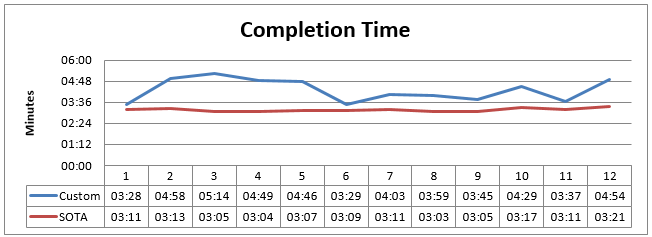
\includegraphics[scale=.8]{Eval2}
\caption{Lap completion differences} \label{fig:timechart}
\end{figure}